\chapter{Implementacija i korisničko sučelje}
		
		
		\section{Korištene tehnologije i alati}

		Komunikacija našem u timu je realizirana korištenjem aplikacija Discord\footnote{https://discord.com/} i Whatsapp\footnote{https://www.whatsapp.com/}.\\ Za izradu UML dijagrama korišten je alat Astah Professional\footnote{http://astah.net/editions/professional}, a kao sustav za upravljanje
izvornim kodom Git\footnote{https://git-scm.com/}. Udaljeni repozitorij projekta je dostupan na web platformi GitLab\footnote{https://gitlab.com/}, a kao razvojno okruženje korišten je IntelliJ IDEA\footnote{https://www.jetbrains.com/idea/} - tvrtke JetBrains\footnote{https://www.jetbrains.com/} te Microsoftov Visual Studio Code\footnote{https://visualstudio.microsoft.com/
}. 
	\\
	 Naša aplikacija napisana je koristeći Spring Framework\footnote{https://spring.io/} i jezik Java\footnote{https://www.oracle.com/java/} za izradu backenda te React\footnote{https://reactjs.org/} - JavaScript library za izradu frontenda. React je open-source, front end, JavaScript knjižnica za izgradnju korisničkog sučelja ili UI komponenti. Održavaju ga Facebook i zajednica pojedinačnih programera i tvrtki. Spring razvojno okruženje je Java platforma koja pruža široki panel opcija kao podrški
razvoju Java aplikacija. Spring rukuje infrastrukturom, tako da programer može usmjeriti svoj
fokus na razvoj aplikacije. \\
Tijekom izrađivanja aplikacije koristili smo i Postman\footnote{https://www.postman.com/} za simuliranje HTTP zahtjeva nad aplikacijom, Google Drive\footnote{https://workspace.google.com/products/drive/} za efikasno dijeljenje organizacijskih informacija i raznih datoteka. 
Baza podataka se nalazi na poslužitelju u oblaku Amazon
Web Services\footnote{https://aws.amazon.com/}.			
			
			\eject 
		
	
		\section{Ispitivanje programskog rješenja}
			
			\textbf{\textit{dio 2. revizije}}\\
			
			 \textit{U ovom poglavlju je potrebno opisati provedbu ispitivanja implementiranih funkcionalnosti na razini komponenti i na razini cijelog sustava s prikazom odabranih ispitnih slučajeva. Studenti trebaju ispitati temeljnu funkcionalnost i rubne uvjete.}
	
			
			\subsection{Ispitivanje komponenti}

			\textbf{Unit testovi za Service sloj}
			\bigskip
			\newline
			Da bi napravili unit testove za svaki razred posebno, koristiti ćemo framework Mockito. Koristiti ćemo ga tako da "simuliramo" rad objekata koji testni razred koristi. @RunWith(MockitoJUnitRunner.class) je anotacija koja se stavlja iznad razreda u kojem su unit testovi. @InjectMocks anotacija nam označuje objekt nad kojim će se vršiti unit test (System under test). @Mock anotacija stvara objekt koji je "lažan", on neće izvoditi svoje normalne metode, već ćemo mu mi kako će se ponašati na svaki poziv metode.
			\bigskip
			\bigskip
			
			\bigskip
			\textbf{UserServiceJpa unit test}
			\bigskip
			
			\textit{listAll()} - metoda listAll() vraća listu korisnika (List<User>). U unit testu stvaramo 3 nova korisnika i simuliramo metodu listAll() da kao rezultat vrati listu od ta 3 korisnika. Zatim pozovemo metodu listAll() i provjerimo vraća li ta metoda dobre podatke nazad.
			
			\textit{registerUser()} - unit testovi za ovu metodu ispituju baca li IllegalArgumentException kada mu predamo korisnika kojemu fali neki od obaveznih podataka za registraciju ili kada već postoji korisnik s tim korisničkim imenom, emailom ili brojem telefona. Ispituje se i radi li metoda sve dobro kada mu predamo korisnika koji ima sve podatke, i ne postoje već korisnici s takvim korisničkim imenom, emailom i brojem telefona.
			
			\textit{updateUser()} - unit testovi za ovu metodu ispituju baca li IllegalArgumentException kada mu predamo korisnika kojemu fali neki od obaveznih podataka za ažuriranje podataka. Ispituje se i radi li metoda očekivano kada se preda korisnik kojemu bi se trebalo bez greške ažurirati podatke.
			
			\textit{findByUsername()} - unit testovi za ovu metodu ispituju baca li IllegalArgumentException kada mu predamo korisničko ime koje je null, vraća li null kada mu predamo korisničko ime za kojeg ne postoji registrirani korisnik i radi li metoda očekivano kada se preda korisničko ime za kojeg postoji registrirani korisnik.
			
			\textit{deleteUser()} - unit testovi za ovu metodu ispituju vraća li ispravno broj obrisanih korisnika. Ukoliko mu predamo korisničko ime za koje ne postoji registrirani korisnik treba vraćati da je broj obrisanih korisnika 0, a ako mu predamo korisničko ime za koje postoji registrirani korisnik treba vraćati da je broj obrisanih korisnika 1.
			
			\textit{getStatistics()} - Ukoliko ne postoje registrirani korisnici pri pozivu ove metode, ona bi trebala vratiti praznu listu. Ako postoje registrirani korisnici, ali ne njih više od dva, metoda bi trebala vratiti samo listu od tog jednog ili dva korisnika, tako da je prvi onaj bolje ocjenjeni. Ako postoji tri ili više registriranih korisnika metoda bi trebala vratiti listu od tri najbolje ocjenjena korisnika. Testira se i u kojem poretku je metoda vratila najbolje ocijenjene korisnike, tu se testira je li dobro implementirano sortiranje korisnika.
			
			\bigskip
			\bigskip
			\textbf{RatingServiceJpa unit test}
			\bigskip
			
			\textit{calculateAverageRatingForUser()} - Ukoliko se preda korisnik čije korisničko ime nema registrirano u bazi podataka baca se NonexistingUserReferencedException. Ako postoji korisnik, ali nema nikakvih ocjena za njega, metoda bi trebala vratiti ocjenu 0.0 . Testira se i računa li metoda ispravno prosječnu ocjenu za korisnika koji postoji i za kojega ima više ocjena spremljenih u bazi.
			
			\bigskip
			\bigskip
			\textbf{RequestServiceJpa unit test}
			\bigskip
			
			\textit{addRequest()} - Ako se metodi preda zahtjev čiji je autor postavljen na null, metoda bi trebala postaviti ulogiranog korisnika kao autora zahtjeva. Ako adresa zahtjeva ne sadrži opis, x kordinatu ili y kordinatu, metoda bi trebala baciti IllegalArgumentException. Ako je predan zahtjev koji je potpun i točan metoda bi trebala uspješno dodati zahtjev.
			
			\bigskip
			\begin{figure}[H]
				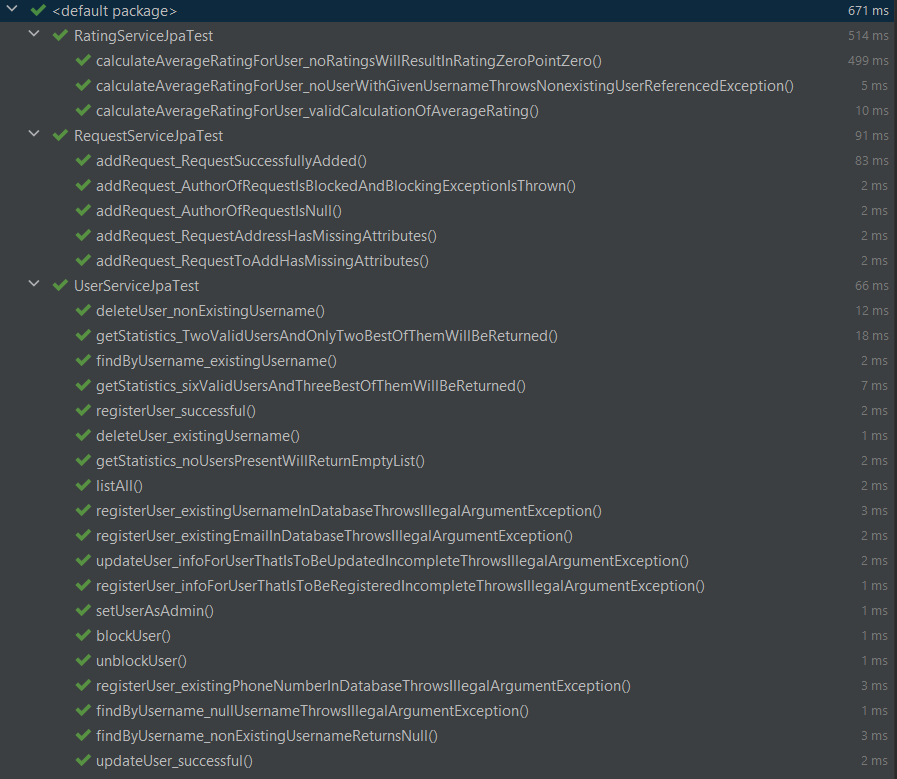
\includegraphics[scale=0.8]{slike/unit_testovi.png}
				\centering
				\caption{Rezultati unit testova}
				
			\end{figure}
			
			
			\subsection{Ispitivanje sustava}
			
			Za ispitivanje sustava korišten je alat za automatizirano testiranje Selenium WebDriver. Ispitni slučajevi pisani
			su u jeziku Java. \newline
			
			Cilj ispitivanja sustava je ispitati ponašanje sustava u cjelini, onako kako ga vidi 
			korisnik aplikacije te dostupnost svih funkcionalnosti koje korisnik može koristiti.
			Napisani ispitni slučajevi prije svega su ispitivali pravilan izgled komponenti i funkcionalnosti koje se nude kroz korisničko sučelja
			u ovisnosti o stanju sustava, stanju pojedinog zahtjeva i ovlastima korisnika koji je prijavljen u sustav.
			Testiranje je koristilo dva korisnika već registrirana u sustav, jednog s ovlastima običnog korisnika i drugog s ovlastima administratora.\newline 
			
			Komponente koje najviše ovise o ovlastima i stanju sustava su komponenta za prikaz pojedinog zahtjeva i komponenta profila korisnika.
			Za primjer, funkcionalnosti rada sa zahtjevima testiraju metode:
			\begin{packed_enum}
				
				\item \textit{createRequestExpectedBehaviour()} - očekivani unos u formu zahtjeva
				\item \textit{createRequestNoTitle()} - neispravan unos u formu zahtjeva
				\item \textit{viewNonAuthoredRequest()} - prisutnost komponenti za javljanje na zahtjev
				\item \textit{viewAuthoredRequest()} - prisutnost komponenti za blokiranje zahtjeva
				\item \textit{viewAuthoredRequestWithPotentialHandlers()} - prisutnost komponenti za pregled potencijalnih izvršitelja te sam pregled
				
			\end{packed_enum}
			
		
			
			Testni slučajevi fokusirali su se na različite situacije i rubne slučajeve u prikazu i funkcionalnostima.
			Rubni slučajevi poput pogrešnog unosa u formu ili nedostatka nekog unosa se u aplikaciji signaliziraju različitim porukama o pogrešci. 
			Testne metode za takve slučajeve prije svega su se fokusirali na traženje odgovarajuće poruke o pogrešci.
			Konkretan primjer za to su testni slučajevi unosa pogrešnih korisničkih podataka u formu za prijavu. \newline 
			
			Neimplementirana funkcionalnost koja je također testirana je traka za pretraživanje. 
			Testom je pokazano da akcijama nad njom se ne mjenja stanje sustava i ne remeti se normalan tijek funkcioniranja aplikacije. \newline
			
			Glavnu prepreku za automatizaciju ispitivanja sustava predstavljala je priroda testiranog sustava. 
			Sustav se sastoji od brojnih aktivnosti koje se mogu izvoditi samo jednom, poput javljanja na pojedini zahtjev ili 
			biranja izvršitelja za zahtjev te aktivnosti koje zahtjevaju slijednu interakciju više korisnika.
			Takve akcije teško je automatizirano ispitivati zato što to neminovno u sustavu akumulira velik broj zahtjeva samo za testiranje 
			ili testove nije moguće ponavljati više puta, čime se u potpunosti gubi njihova svrha.
			Stoga su navedene funkcionalnosti izostavljene iz automatiziranog ispitvanja alatom Selenium i odrađene ručno.
			
			
			
			
			\begin{figure}[H]
				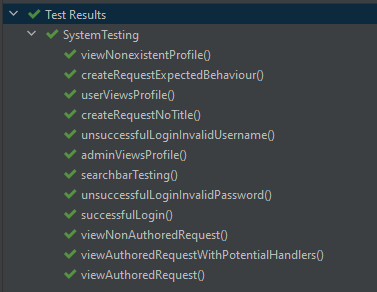
\includegraphics[scale=1.2]{slike/selenium-testing.png}
				\centering
				\caption{Rezultati testova sustava}
				
			\end{figure}
			
			 
			
			\eject 
		
		
		\section{Dijagram razmještaja}
			
			Na slici 5.1 nalazi se dijagram razmještaja koji prikazuje raspored programske podrške aplikaciji unutar sklopovlja.
			
			Sa strane korisnika aplikacije, sklopovlje predstavlja njegovo računalo, mobilni telefon ili bilo koji drugi uređaj s pristupom internetu i instaliranim browserom.
			Internetski browser zadužen je za uspostavu konekcije sa poslužiteljem koja će omogućiti slanje i posluživanje zahtjeva.
			Sa strane poslužitelja sklopovlje predstavlja serversko računalo.
			Dvije glavne usluge koje se nalaze na serverskom računalu su baza podataka i web server koje su nužne za posluživanje zahtjeva.
			
			Komunikacija između korisnika i poslužitelja vrši se putem \textit{stateless} HTTP protokola. 
			Tijekom slanja zahtjeva serveru, korisnikov browser ima otvorenu jednu HTTP vezu prema serveru.
			S druge strane server može posluživati više zahtjeva iz više različitih izvora te stoga može imati i više aktivnih HTTP veza.
			
			\begin{figure}[h]
				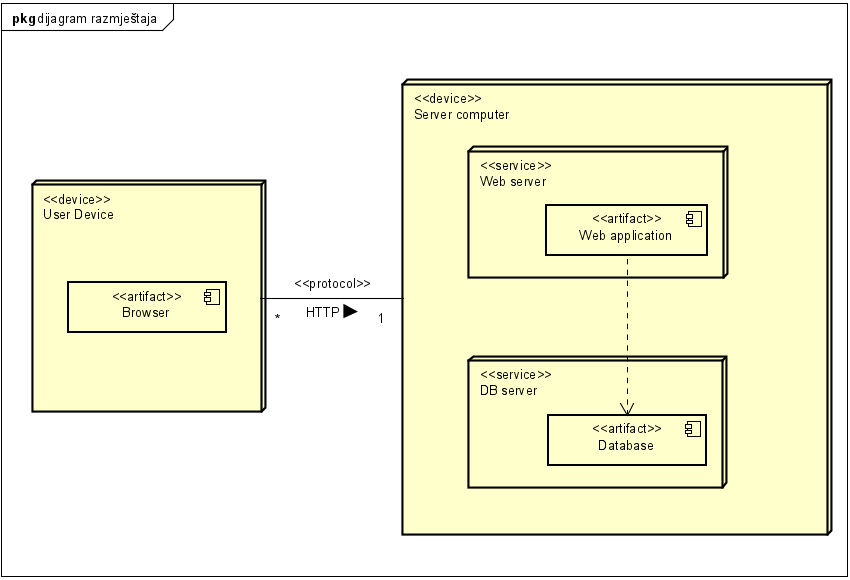
\includegraphics[height=0.5\textheight]{dijagramRazmjestaja}
				\caption{Dijagram razmještaja}
			\end{figure} 
			
			\eject 
		
		\section{Upute za puštanje u pogon}
		
			\textbf{\textit{dio 2. revizije}}\\
		
			 \textit{U ovom poglavlju potrebno je dati upute za puštanje u pogon (engl. deployment) ostvarene aplikacije. Na primjer, za web aplikacije, opisati postupak kojim se od izvornog kôda dolazi do potpuno postavljene baze podataka i poslužitelja koji odgovara na upite korisnika. Za mobilnu aplikaciju, postupak kojim se aplikacija izgradi, te postavi na neku od trgovina. Za stolnu (engl. desktop) aplikaciju, postupak kojim se aplikacija instalira na računalo. Ukoliko mobilne i stolne aplikacije komuniciraju s poslužiteljem i/ili bazom podataka, opisati i postupak njihovog postavljanja. Pri izradi uputa preporučuje se \textbf{naglasiti korake instalacije uporabom natuknica} te koristiti što je više moguće \textbf{slike ekrana} (engl. screenshots) kako bi upute bile jasne i jednostavne za slijediti.}
			
			
			 \textit{Dovršenu aplikaciju potrebno je pokrenuti na javno dostupnom poslužitelju. Studentima se preporuča korištenje neke od sljedećih besplatnih usluga: \href{https://aws.amazon.com/}{Amazon AWS}, \href{https://azure.microsoft.com/en-us/}{Microsoft Azure} ili \href{https://www.heroku.com/}{Heroku}. Mobilne aplikacije trebaju biti objavljene na F-Droid, Google Play ili Amazon App trgovini.}
			
			
			\eject 